\titre{}
\theme{fonctions}
\auteur{Nathan Scheinmann}
\niveau{1M}
\source{ns}
\type{serie}
\piments{2}
\pts{}
\annee{2425}

\contenu{
	\tcblower

\begin{minipage}[t]{0.54\textwidth}{
		\vspace{0pt}
	Ci-contre les représentations graphiques des fonctions $f,g,h$. À l'aide de ces représentations réponds aux questions suivantes.	
	\begin{enumerate}
		\item Déterminer
	\begin{multicols}{3}
		\begin{enumerate}[wide, labelwidth=!,label=,labelindent=0pt]
				\item $f(-3)=$
				\item $g(-2)=$
				\item $f(1)=$
				\item $h(1)$=
				\item $f(0)=$
				\item $g(0)=$
			\end{enumerate}
		\end{multicols}
	\item Si $\ldots$
        \begin{multicols}{2}
		\begin{enumerate}[wide, labelwidth=!,label=,labelindent=0pt]
			\item $f(x)=1$, alors $x=$
			\item $h(x)=5$, alors $x=$
			\item $h(x)=2$, alors $x=$
			\item $g(x)=-2$, alors $x=$
		\end{enumerate}
    \end{multicols}
\item Le point $(-4;0)$ appartient-il au graphe de $h$? Le point $(1:0)$ appartient-il au graphe de $f$?
	\end{enumerate}
		}
		\end{minipage}
		\hfill
		\begin{minipage}[t]{0.45\textwidth}{
		\vspace{0pt}
\begin{center}
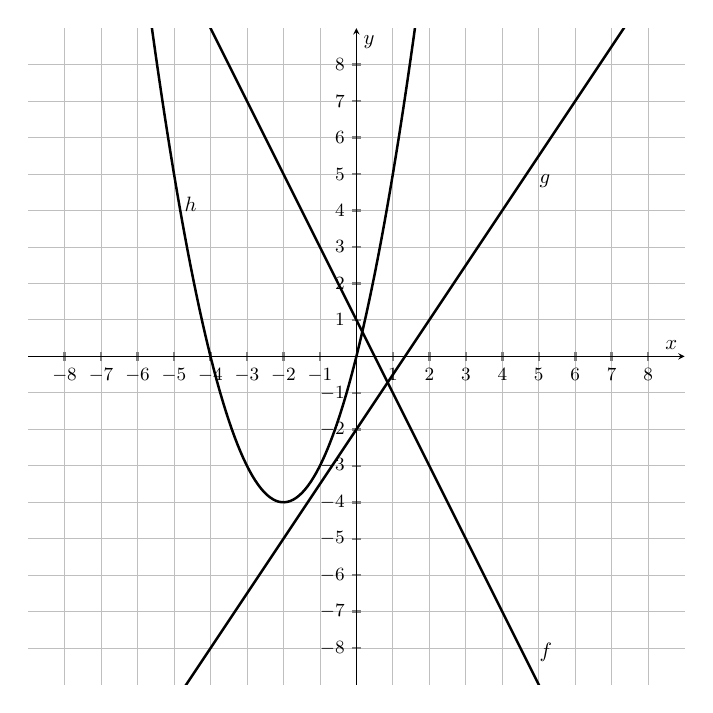
\begin{tikzpicture}[scale=0.75]
\begin{axis}[
  axis lines=center,
  grid=major,
  width=5in,
height=5in,
  xmin=-8,
  xmax=8,
  ymin=-8,
  ymax=8,
  xlabel=$x$,
  ylabel=$y$,
  enlargelimits={abs=1},
  xtick={-8,-7,...,8},
  ytick={-8,-7,...,8},
  xlabel style={at={(rel axis cs:1,0.5)}},
  ylabel style={at={(rel axis cs:0.5,1)}},
  tick style={very thick},
  ticklabel style={font=\small},
  legend style={
  at={(rel axis cs:1,1)},
  anchor=north west,
  draw=none,
  inner sep=0pt,
  fill=gray!10}
]

\addplot [very thick,domain=-8:8,samples=200] {-2*x+1} node [above right,pos=0.8] {$f$};
%\addlegendentry {$f(x)=...$};
\addplot[black,very thick,domain=-8:8,samples=200]{3/2*x-2}  node[below right,pos=0.8] {$g$};
\addplot[black,very thick,domain=-8:8,samples=200]{x^2+4*x}  node[below right,pos=0.2] {$h$};
%\addlegendentry{$g(x)=...$};
\end{axis}
\end{tikzpicture}
\end{center}	
		}
		\end{minipage}
\smallskip
}
\correction{
	\tcblower
	\begin{tasks}
		\task $f(-3)=7, f(1)=-1, f(0)=1, g(-2)=-5, h(1)=5, g(0)=-2$
		\task $f(x)=1\implies x=0, h(x)=2 \implies x\simeq 0,5 \text{ ou } x\simeq -4,5, h(x)=5\implies x=-5 \text{ ou } x=1, g(x)=-2\implies x=0$.
		\task Oui, non.
	\end{tasks}

}

